\chapter{Presentation: Poster, Demo, Documentation, and Ethics}
\label{ch:presentation}

\begin{quote}
\emph{``If you can't explain it simply, you don't understand it well enough.''} A capstone lives or dies in the 15~minutes you have to make a stranger care, trust, and remember what you built and why it matters.
\end{quote}

\noindent\fbox{\parbox{\dimexpr\linewidth-2\fboxsep-2\fboxrule}{%
\textbf{From zero: no prior presentation training assumed.} We define \emph{poster}, \emph{demo}, \emph{documentation}, and \emph{research ethics} from first principles---intuition and checklists before polish. We assume a working system (Ch.~5--7) and a written report (Ch.~7) to communicate. No design background needed.}}

\vspace{0.4em}

\section*{Learning Outcomes}
After this chapter you will be able to:
\begin{enumerate}[label=(L\arabic*)]
    \item design a poster that tells a complete story in 90~seconds of scanning;
    \item deliver a live demo with a rehearsed script, rollback plan, and risk mitigation;
    \item produce user and developer documentation that enables handover without your presence;
    \item reason about ethics: privacy (PDPA), consent, attribution, and sustainability of your artefact;
    \item handle Q\&A with honesty about limitations and a constructive future-work narrative.
\end{enumerate}

% ============================================================
\section{The Poster: A 90-Second Story}
\label{sec:poster}

A poster is not a shrunken report. It is a \emph{visual abstract} for a busy assessor walking a hall of 60 posters. They will give you 90~seconds of scanning and 3~minutes of conversation. Design for that.

\textbf{Structure in six blocks:} (1)~Title + team + stakeholder logo, (2)~Problem (one sentence + pain number), (3)~Solution (one architecture sketch + 2 screenshots), (4)~Evidence (one metrics table or before/after chart), (5)~What we learned (1 limitation + 1 trade-off), (6)~QR codes (demo video, repo, live URL). Grid the poster into 3 columns $\times$ 2 rows; use whitespace deliberately.

\begin{figure}[h]
\centering
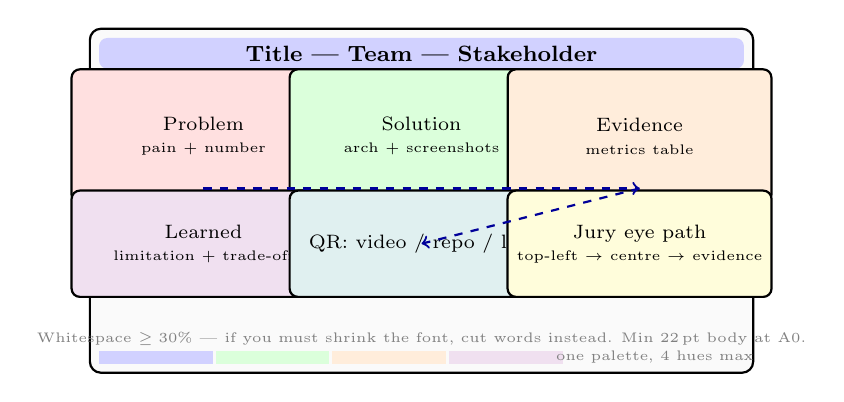
\begin{tikzpicture}[scale=0.78, every node/.style={font=\scriptsize},
  block/.style={draw,thick,rounded corners=3pt,align=center,minimum height=1.0cm}]
  % poster frame
  \draw[thick,rounded corners=4pt,fill=gray!4] (0,0) rectangle (10.8,5.6);
  % header
  \fill[blue!18,rounded corners=3pt] (0.15,4.95) rectangle (10.65,5.45);
  \node[font=\footnotesize\bfseries] at (5.4,5.20) {Title --- Team --- Stakeholder};
  % row 1: problem, solution, evidence
  \node[block,fill=red!12,minimum width=3.35cm,minimum height=1.7cm] at (1.85,3.85) {Problem\\{\tiny pain + number}};
  \node[block,fill=green!14,minimum width=3.35cm,minimum height=1.7cm] at (5.40,3.85) {Solution\\{\tiny arch + screenshots}};
  \node[block,fill=orange!14,minimum width=3.35cm,minimum height=1.7cm] at (8.95,3.85) {Evidence\\{\tiny metrics table}};
  % row 2: learning, QR, design tip
  \node[block,fill=violet!12,minimum width=3.35cm,minimum height=1.35cm] at (1.85,2.10) {Learned\\{\tiny limitation + trade-off}};
  \node[block,fill=teal!12,minimum width=3.35cm,minimum height=1.35cm] at (5.40,2.10) {QR: video / repo / live};
  \node[block,fill=yellow!14,minimum width=3.35cm,minimum height=1.35cm] at (8.95,2.10) {Jury eye path\\{\tiny top-left $\to$ centre $\to$ evidence}};
  % eye path
  \draw[->,thick,blue!60!black,dashed] (1.85,3.0) -- (5.40,3.0) -- (8.95,3.0);
  \draw[->,thick,blue!60!black,dashed] (8.95,3.0) -- (5.40,2.10);
  % whitespace note
  \node[font=\tiny,gray,align=center] at (5.4,0.55) {Whitespace $\ge 30$\% --- if you must shrink the font, cut words instead. Min 22\,pt body at A0.};
  % colour bar
  \fill[blue!18] (0.15,0.15) rectangle (2.0,0.35); \fill[green!14] (2.05,0.15) rectangle (3.9,0.35);
  \fill[orange!14] (3.95,0.15) rectangle (5.8,0.35); \fill[violet!12] (5.85,0.15) rectangle (7.7,0.35);
  \node[font=\tiny,gray] at (9.2,0.25) {one palette, 4 hues max};
\end{tikzpicture}
\caption{Poster grid: header plus five content blocks with a dashed eye path (problem $\to$ solution $\to$ evidence). Colour distinguishes block type; whitespace and font floor protect readability at 1.5\,m.}
\label{fig:poster-grid}
\end{figure}

\textbf{Typography and colour.} One sans-serif family, two weights, four colours max. Body $\ge 22$\,pt at A0; headings 1.4$\times$. Use a single accent colour for all callouts so the eye knows what is important. Test readability by printing A4 at 25\% scale and reading from 1.5\,m.

\textbf{Common failures:} wall of text, 8\,pt screenshots, no evidence (``users liked it'' without $n$ or SUS), and a system diagram that is an undecorated box-and-arrow with no labels. Replace adjectives with numbers.

% ============================================================
\section{The Demo: Theatre with a Rollback Plan}
\label{sec:demo}

A demo is theatre: rehearsed, timed, and resilient. Structure a 10-minute capstone demo as follows:

\begin{enumerate}[leftmargin=*,itemsep=0.25em]
    \item \textbf{Hook (1\,min):} one real user pain, one outcome promise, one stakeholder quote.
    \item \textbf{Live walk (6\,min):} two user stories end-to-end (happy path + one error recovery), narrated as a user, not as a developer listing features.
    \item \textbf{Evidence (2\,min):} one slide---metric before/after, SUS, or risk that was mitigated by design (cite report section).
    \item \textbf{Close (1\,min):} what you are proud of, one honest limitation, and one concrete next step if given another sprint.
\end{enumerate}

Pre-demo checklist: fresh incognito browser, seeded demo data, stable Wi-Fi plus phone hotspot backup, backup video of the same flow (30\,s, muted, with captions), and a tagged release of the demo build so you can rollback in one command.

\begin{lstlisting}[language=Python,caption={Demo script as executable checklist: each step is timed, owned, and has a fallback.},label={lst:demo-script}]
demo_script = [
    {"t": "0:00", "who": "Asha", "says": "Polyclinic A loses 18% of slots to no-shows.",
     "does": "Show poster problem block; 90s scan."},
    {"t": "1:00", "who": "Ben",  "says": "As a patient I scan QR and see my ETA.",
     "does": "Live: scan QR -> live queue (seed: 5 ahead) -> SMS arrives",
     "fallback": "Play backup_video/eta_flow_30s.mp4"},
    {"t": "4:00", "who": "Chen", "says": "If I cancel late, the system protects the queue.",
     "does": "Live: cancel after acceptance -> 'Too late' error (US-07)",
     "fallback": "Screenshot + Gherkin scenario on slide"},
    {"t": "7:00", "who": "Dana", "says": "Pilot evidence: p95 340ms, SUS 78 (n=8).",
     "does": "Show Report Fig. 7.1; cite NFR-03 trace matrix"},
    {"t": "9:00", "who": "Asha", "says": "Honest limit + next sprint: PDPA audit + EHR API.",
     "does": "Close with QR to live URL + repo tag v0.4.0-demo"},
]
# rehearse 3x with timer; cut to 9:30 to leave 30s buffer
\end{lstlisting}

Handle Q\&A with ``what we built, what we measured, what we would change.'' If you do not know, say so and offer to follow up---bluffing is remembered longer than a gap. Never apologise for scope you deliberately deferred; frame it as a MoSCoW choice with stakeholder agreement.

\begin{figure}[h]
\centering
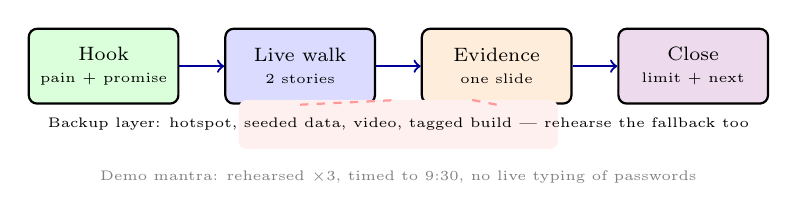
\begin{tikzpicture}[scale=0.78, every node/.style={font=\scriptsize},
  stage/.style={draw,thick,rounded corners=3pt,minimum width=1.9cm,minimum height=0.95cm,align=center}]
  \node[stage,fill=green!14] (hook) at (0,0) {Hook\\{\tiny pain + promise}};
  \node[stage,fill=blue!14] (live) at (3.2,0) {Live walk\\{\tiny 2 stories}};
  \node[stage,fill=orange!14] (evidence) at (6.4,0) {Evidence\\{\tiny one slide}};
  \node[stage,fill=violet!14] (close) at (9.6,0) {Close\\{\tiny limit + next}};
  \draw[->,thick,blue!60!black] (hook) -- (live);
  \draw[->,thick,blue!60!black] (live) -- (evidence);
  \draw[->,thick,blue!60!black] (evidence) -- (close);
  % backup underlay
  \fill[red!6,rounded corners=3pt] (2.2,-1.35) rectangle (7.4,-0.55);
  \node[font=\tiny,align=center] at (4.8,-0.95) {Backup layer: hotspot, seeded data, video, tagged build --- rehearse the fallback too};
  \draw[dashed,red!40,thick] (live.south) -- (4.8,-0.55);
  \draw[dashed,red!40,thick] (evidence.south) -- (6.0,-0.55);
  \node[font=\tiny,gray,align=center] at (4.8,-1.80) {Demo mantra: rehearsed $\times 3$, timed to 9:30, no live typing of passwords};
\end{tikzpicture}
\caption{Demo arc with a backup layer beneath the live walk. The dashed tether reminds the team that every live step has a pre-recorded twin that can take over in under 10~seconds.}
\label{fig:demo-arc}
\end{figure}

% ============================================================
\section{Documentation and Ethics: Handover with Conscience}
\label{sec:documentation-ethics}

Code without documentation is a liability the day you graduate. Produce two documents:

\textbf{User guide:} task-oriented (``How to cancel an order''), not feature-oriented; each task is a numbered list with screenshots at decision points, plus a one-page troubleshooting FAQ. Test it by asking a non-team member to complete the tasks unaided.

\textbf{Developer handover:} architecture sketch (Fig.~\ref{fig:layered-architecture} updated), setup steps that work from zero (\texttt{git clone} $\to$ \texttt{docker compose up} $\to$ green CI), environment variables, seed data, known limitations, and a 30-day maintenance plan (who to contact, backup schedule). Archive the traceability matrix so a future team can answer ``why was this built this way?''

\begin{figure}[h]
\centering
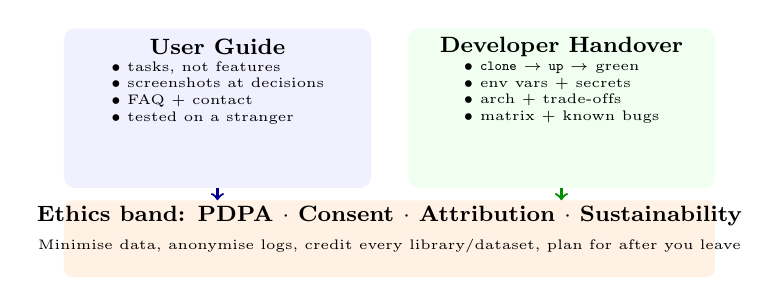
\begin{tikzpicture}[scale=0.78, every node/.style={font=\scriptsize}]
  % two docs side by side
  \fill[blue!6,rounded corners=4pt] (0,0) rectangle (5.0,2.6);
  \fill[green!6,rounded corners=4pt] (5.6,0) rectangle (10.6,2.6);
  \node[font=\footnotesize\bfseries] at (2.5,2.30) {User Guide};
  \node[font=\tiny,align=left] at (2.5,1.55) {$\bullet$ tasks, not features\\$\bullet$ screenshots at decisions\\$\bullet$ FAQ + contact\\$\bullet$ tested on a stranger};
  \node[font=\footnotesize\bfseries] at (8.1,2.30) {Developer Handover};
  \node[font=\tiny,align=left] at (8.1,1.55) {$\bullet$ \texttt{clone} $\to$ \texttt{up} $\to$ green\\$\bullet$ env vars + secrets\\$\bullet$ arch + trade-offs\\$\bullet$ matrix + known bugs};
  % ethics band
  \fill[orange!10,rounded corners=3pt] (0,-1.45) rectangle (10.6,-0.20);
  \node[font=\footnotesize\bfseries] at (5.3,-0.45) {Ethics band: PDPA $\cdot$ Consent $\cdot$ Attribution $\cdot$ Sustainability};
  \node[font=\tiny,align=center] at (5.3,-0.95) {Minimise data, anonymise logs, credit every library/dataset, plan for after you leave};
  \draw[->,thick,blue!55!black] (2.5,0) -- (2.5,-0.20);
  \draw[->,thick,green!55!black] (8.1,0) -- (8.1,-0.20);
\end{tikzpicture}
\caption{Two documentation audiences plus the ethics band that constrains both. User guide serves the stakeholder; handover serves the next team; ethics serves everyone the system touches.}
\label{fig:docs-ethics}
\end{figure}

\textbf{Ethics.} (i)~\emph{Privacy (PDPA):} collect only what you need, justify each field, store with access control, set a retention deadline, and honour deletion requests. (ii)~\emph{Consent:} written, informed, voluntary, and withdrawable---separate from grading. (iii)~\emph{Attribution:} cite datasets, libraries, and AI assistance; respect licences (MIT/Apache vs.\ GPL). (iv)~\emph{Sustainability:} who pays for hosting after handover? Document cost and a shutdown or transfer plan so the system does not become abandonware with live personal data.

Sustainability is an ethical issue: deploying a system that handles personal data without a maintenance owner is irresponsible. Agree ownership in writing before final demo.

% ============================================================
\section{Handling Q\&A and Lifelong Lessons}
\label{sec:qanda}

The Q\&A after your demo is not cross-examination; it is evidence that you can reason beyond rehearsed lines. Three question archetypes recur:

\begin{itemize}
    \item \textbf{Design rationale:} ``Why X over Y?'' Answer with trade-offs and numbers: ``We chose a modular monolith because with one DB and four people, microservices would have added 2\,weeks of DevOps for no scaling benefit (Ch.~3). If users grew 10$\times$, we would extract the notification service first.''
    \item \textbf{Evidence challenge:} ``Your p95 was 620\,ms, above the 500\,ms target. Is that failure?'' Own the miss: ``Verdict is Fail against NFR-03 (Table~\ref{tab:results-example} analogue). Root cause is N+1 queries on the dashboard; fix is eager batch fetch, expected $-$40\% latency. We report it as a limitation, not a hidden miss.''
    \item \textbf{Ethics and handover:} ``Who maintains this after graduation?'' Point to the handover: ``Owner is Prof.~Tan's lab, cost S\$12/month on Fly.io, documented shutdown steps if unmaintained for 6~months (ethics band, Fig.~\ref{fig:docs-ethics}).''
\end{itemize}

\begin{remark}[Future-work framing]
Never end with ``if we had more time we would...'' without scope. Instead: ``Given one more sprint we would (1) add PDPA audit logging (2~pts), (2) run a field test in the hawker centre on 4G ($n=10$), and (3) cache dashboard queries---in that order, because audit is Must for deployment and cache addresses the measured NFR miss.''
\end{remark}

\begin{remark}[Poster printing checklist]
Export at 300\,dpi, embed fonts, proof colours on the actual printer (projector vs.\ print differ), and bring Blu Tack plus a 2-page handout with the QR links. Arrive 20\,minutes early to hang and test sightlines. Check that QR codes scan from 1\,m and that the live URL is still the tagged demo build, not a dev branch that may be mid-migration.
\end{remark}

The capstone's lasting value is not the code (which will be rewritten) but the habits: traceable decisions, honest evaluation, and empathy for the next maintainer and the user who must live with what you built.

\begin{remark}[Ethics review prompt]
Before collecting any personal data, ask: Do we need this field to satisfy a Must requirement? Can we pseudonymise it? How long must we keep it, and what is the deletion trigger? Document the answers in the proposal; PDPA compliance is design, not paperwork added after the system works.
\end{remark}

\begin{remark}[Stakeholder thank-you]
Close the loop: send stakeholders a one-page summary (problem, solution, evidence, next owner) and archive their acknowledgement. Gratitude and a clean handover turn a semester project into a relationship you can cite in interviews and future work.
\end{remark}

% ============================================================
\section{Exercises}
\label{sec:ch08-exercises}
\begin{enumerate}[label=E8.\arabic*, leftmargin=*, itemsep=0.6em]
    \item \textbf{Poster critique.} Given a poster crammed with 900 words in 10\,pt, no whitespace, and 6\,pt screenshots, apply Fig.~\ref{fig:poster-grid} to redesign: state what to cut, what to enlarge, and where evidence goes. Justify with the 90-second scan budget.
    \item \textbf{Demo script + risk.} Write a 9:30 script for your capstone using Listing~\ref{lst:demo-script} as template. List three live-demo risks (Wi-Fi, data, auth expiry), the fallback for each, and the one-line cue that triggers the fallback without audience panic.
    \item \textbf{Documentation test.} Draft the ``Setup from zero'' page of your developer handover (clone, env, compose, seed, CI). Then design a 20-minute test where a classmate follows it unaided; list the three failure signals that prove your doc is incomplete.
    \item \textbf{PDPA data audit.} Your app stores name, phone, matric, and location. For each field, state purpose, legal basis, retention, and deletion mechanism. Which fields would you drop or pseudonymise to minimise data and still meet Must requirements?
    \item \textbf{Q\&A preparation.} Prepare honest answers for: (a) ``Why did you choose a monolith over microservices?'' (b) ``Your p95 was 620\,ms, not 500\,ms---is the project a failure?'' (c) ``Who maintains this after you graduate and at what cost?'' Tie each answer to Ch.~3, Ch.~7, and the ethics band respectively.
\end{enumerate}
\begin{remark}[Final 48-hour checklist]
Poster printed and QR-tested, demo video rendered, live URL on tagged release, handout PDF, handover docs linked, and one full dress rehearsal with timer and fallback trigger. Sleep 7 hours; a rested team demos better than a cramming one. Check venue: HDMI vs.\ USB-C, microphone, and that your font is embedded---borrowed laptops drop custom fonts.
\end{remark}
% End of Chapter 8
